% Opcje klasy 'iithesis' opisane sa w komentarzach w pliku klasy. Za ich pomoca
% ustawia sie przede wszystkim jezyk oraz rodzaj (lic/inz/mgr) pracy.
\documentclass[shortabstract]{iithesis}

\usepackage[utf8]{inputenc}
\usepackage{hyperref}
\usepackage{graphicx}
%%%%% DANE DO STRONY TYTUŁOWEJ
% Niezaleznie od jezyka pracy wybranego w opcjach klasy, tytul i streszczenie
% pracy nalezy podac zarowno w jezyku polskim, jak i angielskim.
% Pamietaj o madrym (zgodnym z logicznym rozbiorem zdania oraz estetyka) recznym
% zlamaniu wierszy w temacie pracy, zwlaszcza tego w jezyku pracy. Uzyj do tego
% polecenia \fmlinebreak.
\polishtitle    {Aplikacja mobilna do zarządzania i tworzenia\fmlinebreak  interaktywnych notatek}
\englishtitle   {A mobile application to manage and create interactive notes}
\polishabstract {TODO: streszczenie po polsku\ldots}
\englishabstract{TODO: streszczenie po angielsku\ldots}
% w pracach wielu autorow nazwiska mozna oddzielic poleceniem \and
\author         {Bartosz Sobocki}
% w przypadku kilku promotorow, lub koniecznosci podania ich afiliacji, linie
% w ponizszym poleceniu mozna zlamac poleceniem \fmlinebreak
\advisor        {dr Marcin Młotkowski}
%\date          {}                     % Data zlozenia pracy
% Dane do oswiadczenia o autorskim wykonaniu
%\transcriptnum {}                     % Numer indeksu
%\advisorgen    {dr. Marcina Młotkowskiego} % Nazwisko promotora w dopelniaczu
%%%%%

%%%%% WLASNE DODATKOWE PAKIETY
%
%\usepackage{graphicx,listings,amsmath,amssymb,amsthm,amsfonts,tikz}
%
%%%%% WŁASNE DEFINICJE I POLECENIA
%
%\theoremstyle{definition} \newtheorem{definition}{Definition}[chapter]
%\theoremstyle{remark} \newtheorem{remark}[definition]{Observation}
%\theoremstyle{plain} \newtheorem{theorem}[definition]{Theorem}
%\theoremstyle{plain} \newtheorem{lemma}[definition]{Lemma}
%\renewcommand \qedsymbol {\ensuremath{\square}}
% ...
%%%%%

\begin{document}

%%%%% POCZĄTEK ZASADNICZEGO TEKSTU PRACY

\chapter{Wprowadzenie}

\section{Cel projektu}

Celem projektu jest wytworzenie aplikacji mobilnej do zarządzania notatkami w interaktywny sposób.
Aplikacja ma umożliwić użytkownikowi prowadzenie i tworzenie notatek pozwalających na edycję tekstu i inncyh elementów znajdujących się w notatce bez konieczności zmian widoków, przełączenia całej zawartości pomiędzy trybem edycji, a trybem użytkowym, czy potrzeby zapisu notatki, aby jej zawartość była dostępna w postaci końcowego efektu.
Graficzny interfejs użytkownika powinien być przystępny i pozwalać na edycję poszczególnych elementów, podczas gdy pozostała zawartość notatki jest wyświetlana w trybie widoku.
Do przechowywania zawartości notatek powinna zostać użyta baza danych, jak również odpowiedni format zapisu dancyh do przechowywania zawartości niebędącej tekstem. 

\section{Opis Aplikacji}

Aplikacja MobiNote służy do zarządzania notatkami w sposób opisany powyżej.
Głównym zamysłem aplikacji jest pomoc korzystającemu w prowadzeniu, tworzeniu i zapisywaniu notatek, w których skład wchodzi nie tylko tekst, ale również przyciski, obrazy, listy, liczniki i różnego rodzaju pomocne widgety.
Aplikacja umożliwia tworzenie i utrzymywanie brudnopisu używanego podczas codziennych czynności, jak również przejrzystych, dopracowanych i przystępnych  notatek.

Wytworzone notatki mogą być używane w formie brudnopisu, między innymi podczas: treningu na siłowni, organizacji przyjęcia, nauki z wykorzystaniem sesji pomodoro, tworzeniu listy zakupów oraz wielu innych codziennych czynności.

Mogą także w przyjemny dla oka sposób przechowywać i wyświetlać informacje przygotowane w celu tworzenia dziennika, notatek do nauki, spisu pomysłów i ważnych myśli, czy tworzenia różnego rodzaju list i opisów, takich jak lista miejsc, które użytkownik chciałby odwiedzić wraz z opisem i zdjęciami miejsc, które chciałby tam zobaczyć.

Interaktywność notatki jest zapewniana poprzez możliwość tworzenia zawartości na bierząco za pomocą klawiatury i dostępnego interfejsu użytkownika.
Uzytkownik może tworzyć styl tekstu za pomocą znaczników dodawanych wewnątrz tekstu w odpowiednich miejscach, podobnie do języka znaczników Markdown.
Dodawając odpowiednie znaczniki w tekście można ustawić wielkość czcionki w danym paragrafie, kursywe, podkreślenie, przekreślenie, a także pogrubienie.
Tekst jest automatycznie dostosowywany wraz z dodaniem znaczników, co pozawala na bierząco obserwować i dostosowywać style i wielkości czcionki do potrzeb korzystającego.

Interfejs użytkownika jest prosty i przejrzysty, posiada motyw ciemny(dark), jasny(light) oraz ułatwiający użytkowanie(easy) dla osób widzących słabiej.

\chapter{Instalacja}

Kod żródłowy aplikacji wraz plikiem \textbf{.apk} można uzyskać pobierając repozytorium \textbf{MobiNote} pod linkiem:
\url{https://github.com/bsobocki/MobiNote}.

\section{Aplikacje z nieznanych źródeł}
Do zaintalowania aplikacji potrzbna jest możliwość instalowania nieznanych aplikacji za pomocą menadżera plików.
Aby ją uruchomić, należy:
\begin{itemize}
    \item otworzyć \textbf{Ustawienia}
    \item w \textbf{Ustawieniach} przejść do sekcji \textbf{Aplikacje}
    \item następnie kliknąć na ikone menu (trzy kropki w prawym górnym rogu)
    \item przejść do opcji \textbf{Dostęp specjalny}
    \item następnie \textbf{Zainstaluj nieznane aplikacje}
    \item wybrać menadżera plików i włączyć dla niego tę opcję
\end{itemize}

\textbf{Ważne!} Dla bezpieczeństwa po zainstalowaniu aplikacji warto ponownie wyłączyć możliwość instalowania aplikacji z nienzanych źródeł, jeśli więcej aplikacji nie będzie w ten sposób instalowane.

\section{Instalacja z pliku apk-release.apk}
Aby zainstalować aplikację na urządzeniu mobilnym z systemem Android:

\begin{itemize}
    \item pobirać repozytorium za pomocą polecenia

    \verb|git clone git@github.com:bsobocki/MobiNote.git|
    \item podłączyć urządzenie i przenieść pliki \textbf{apk-release.apk} do wybranego przez siebie miejsca docelowego na urządzeniu
    \item włączyć możliwość instalacji nienzanych aplikacji (szczegóły powyżej)
    \item w menagerze plików znaleźć miejsce docelowe pliku \textbf{apk-release.apk} i uruchomić
    \item kliknąć \textbf{Zaintaluj}
\end{itemize}

\chapter{Podręcznik Użytkownika}

\section{Strona Domowa}

Po uruchomieniu aplikacji użytkownik zostaje przeniesiony na stronę domową. Znajdzie tam swoje notatki i zeszyty wraz z przyciskiem w prawym dolnym rogu służącego do tworzenia nowej notatki, jak również dodatkowe elementy w menu górnego paska, pozwalające na zmianę motywu, czy reset bazy danych w celu usunięcia wszystkich notatek. 

\begin{figure}[h]
    \centering
    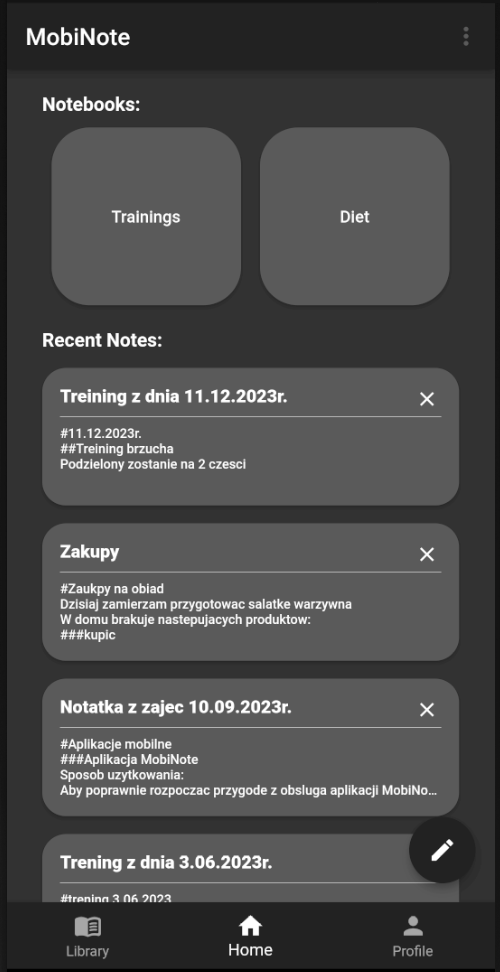
\includegraphics[height=10cm]{images/strona_domowa.png}
    \quad\quad
    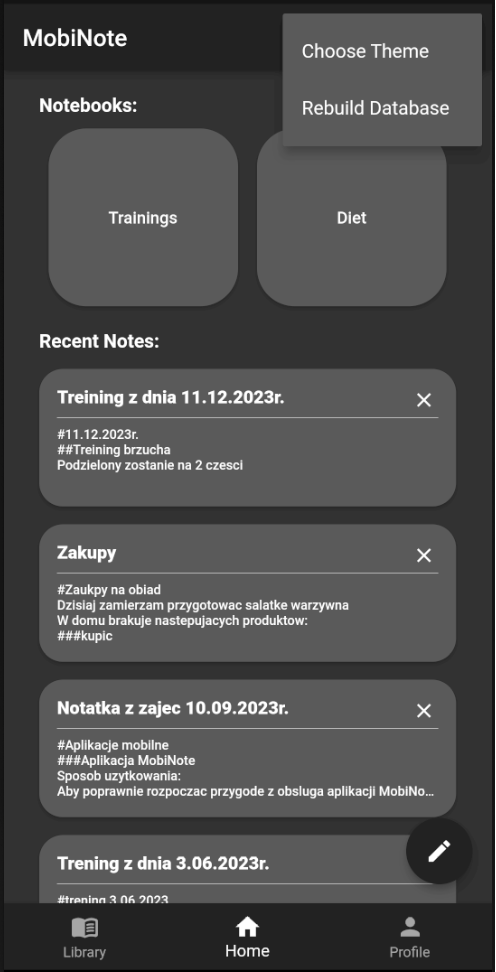
\includegraphics[height=10cm]{images/strona_domowa_opcje.png}
    \caption{Strona domowa aplikacji MobiNote z wybranym motywem \textbf{dark}.}
\end{figure}

\subsection{Opcja \textit{Choose Theme}}

Po uruchomieniu tej opcji wyświetli się okienko dialogowe z wyborem motywu, jakiego użytkownik chciałby użyć. Do wyboru mamy trzy mowtywy: \textbf{dark}, \textbf{light} oraz \textbf{easy}.

Motywy \textbf{dark} oraz \textbf{light} służą, jako główne motywy aplikacji, zachowując te same wielkości elementów tekstu i całej aplikacji.
Dla osób mających problemy z widocznością tekstu przy domyślnych ustawieniach wielkości i kolorów aplikacji przygotowany został mowtyw \textbf{easy}.
Motyw ten cechują kontrastujące ze sobą kolory, jak również zwiększone rozmiary czcionek, ikon, przycisków i paska narzędzi.

\begin{figure}[h]
    \centering
    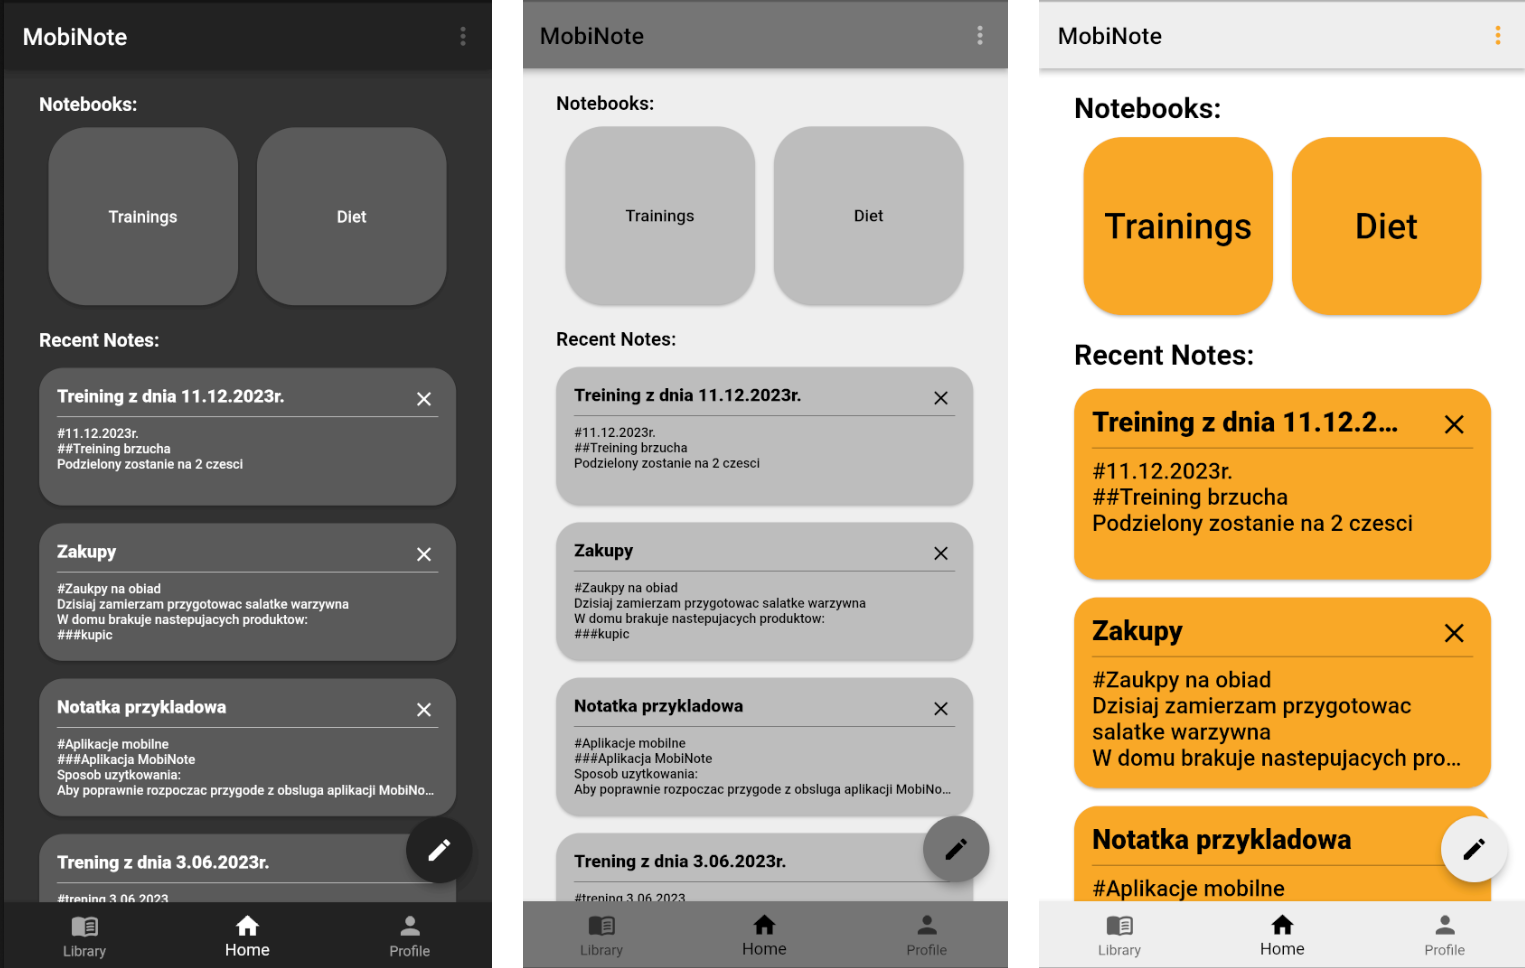
\includegraphics[height=8.5cm]{images/strona_domowa_motywy.png}
    \caption{Porównanie motywów na tej samej stronie domowej.}
\end{figure}

\subsection{Opcja \textit{Rebuild Database}}

Opcja ta otwiera okno dialogowe z pytaniem o to, czy na pewno chcemy wykonać tę przebudowanie bazy danych. Po zatwierdzeniu baza danych jest usuwana i budowana.

\subsection{Zeszyty}

Pod etykietą \textbf{\textit{Notebooks:}} widnieją dwa przyciski \textbf{Trainings} oraz \textbf{Diet}. Są to roboczo dodane przyciski, które są przygotowane pod rozszerzenie aplikacji w przyszłości o możliwość układania notatek w zeszyty, dla lepszej organizacji, a także wprowadzać etykiety.
Pomysł ten zostanie omówiony w rozdziale \textbf{Rozszerzenie Funkcjonalnosći aplikacji}.

\subsection{Notatki}

Kolejnym elementem strony domowej jest lista notatek znajdująca się pod etykietą \textbf{\textit{Recent Notes:}}. Każdy element zawiera tytuł oraz pierwsze cztery surowe linie tekstu(zawierające znaki specjalne styli w przypadku paragrafu będącego tekstem, lub string w formacie JSON reprezentujący widget zawarty w danym paragrafie).
W prawym górnym rogu elementów znajduje się przycisk \textbf{X} służący do usunięcia danej notatki z bazy danych.
Po naciśnięciu na dany element użytkownik zostaje przeniesiony do ekranu wyświetlania i edycji wybranej notatki.

W prawym dolnym rogu ekranu widnieje okrągły przycisk z ikoną ołówka.
Po jego naciśnięciu korzystający zostaje przeniesiony do ekranu edycji, gdzie może stworzyć i zapisać nową notatkę.

\section{Strona Edycji Notatki}

Po wybraniu notatki, lub przejściu do tworzenia nowej, na ekranie pojawi się strona edycji notatki. Składa się ona z głównego paska strony, paska narzędzi, oraz edytora.

\subsection{Pasek Strony}

\subsubsection{Przycisk Zapisu i Powrotu}

Aby wyjść i zapisać notatkę korzystający używa przycisku powrotu.
Ważnym jest, aby zamiast systemowych przycisków nawigacyjnych użyć właśnie tego przycisku nawigacyjnego, ponieważ wraz z powrotem do strony domowej zapisuje on notatkę, jeśli ta uległa zmianie.

Za zmianę notatki uważamy:

\begin{itemize}
    \item edycję tekstu w paragrafie tekstowym
    \item edycję widgetu w paragrafie widgetu
\end{itemize}

\textbf{WAŻNE!} Nowa notatka nie zostaje utworzona w momencie otwarcia okna edycji, a dopiero poprzez użycie przycisku powrotu pod warunkiem, ze jej tytuł lub zawartość uległy edycji. Oznacza to, że przejście do edycji nowej notatki, a następnie powrót, nie zapiszą pustej notatki, jednak dodanie i usunięcie znaku umożliwią zapis przy powrocie.

\subsubsection{Edytor tytułu}

Jest to pole tekstowe widniejące zaraz obok \textbf{Przycisku zapisu i powrotu}. Służy ono do edycji tytułu notatki.

\subsubsection{Przycisk zmiany opcji zapisu}

Ostatnim elementem paska jest \textbf{przycisk zmiany opcji zapisu}. Jest to przycisk typu \textbf{switch} domyślnie ustawiony na true. Każdorazowe kliknięcie zmienia jego logiczną wartość.
Wartość \textbf{true} oznacza zapis notatki w przypadku jej edycji, natomiast \textbf{false} oznacza brak zapisu stanu notatki, nawet jeśli została ona zmieniona.

\subsection{Pasek Narzędzi}

W tym pasku znajdują się przyciski oznaczone ikonami.
W aktualnej wersji aplikacji dostępne są dwa przyciski: dodanie obrazu(ikona obrazu), oraz dodanie listy(ikona listy).

\subsubsection{Dodanie obrazu}

Do zawartości notatki można dodawać również obrazy. Aby to zrobić należy kliknąć przycisk z ikoną obrazu na pasku narzędzi edytora notatki, a następnie wybrać z urządzenia zdjęcie, które ma zostać użyte. Zdjęcie zostanie dodane do notatki.

\textbf{Dodanie listy}

Po wybraniu tej opcji na ekranie pojawi się lista złożona początkowo z jednego elementu typu checkbox zawierające również puste pole tekstowe.

\subsection{Edytor Strony}

Edytor strony zajmuje reszę powierzchni ekranu. Jest polem, w którym następuje edycja tekstu oraz widgetów. Aktualny stan wizualny jest odświeżany na bieżąco, dzięki czemu użytkownik obserwuje zmiany jako efekt końcowy w czasie rzeczywistym.


\chapter{Implementacja}

%%%%% BIBLIOGRAFIA

%\begin{thebibliography}{1}
%\bibitem{example} \ldots
%\end{thebibliography}

\end{document}